\section{Theorie}

%Frequenzbereich
\subsection{Frequenzbereiche}
Allgemein kann der Frequenzbereich in vier Bereiche unterteilt werden.
Das menschliche Ohr kann Frequenzen im Bereich von ca. $\SI{16}{\hertz}$ bis ca. $\SI{20}{\kilo\hertz}$ wahrnehmen.
Dieser Bereich wird als Hörschwelle bezeichnet.
Unterhalb der Hörschwelle spricht man vom Infraschall und Oberhalb bis ca. $\SI{1}{\giga\hertz}$ vom Ultraschall.
Frequenzen über $\SI{1}{\giga\hertz}$ werden Hyperschall genannt.

%Doppler-Effekt
\subsection{Doppler-Effekt}
Der Doppler-Effekt beschreibt die Frequenzänderung, welche bei einer relativen Bewegung der Schallquelle und des Beobachter auftritt.
Die Frequenz steigt, sobald der Beobachter sich mit der Geschwindigkeit $v$ auf die ruhende Quelle zubewegt ($\nu_{kl}$) und sinkt wenn dieser sich von der Quelle entfernt ($\nu_{gr}$)
\begin{equation}
    \nu_{kl/gr} = \frac{\nu_0}{1\mp \frac{v}{c}} \, .
    \label{eqn:doppler_beobachter}
\end{equation}
Dabei steht $c$ für die Lichtgeschwindigkeit und $\nu_0$ für die Ausgangsfrequenz.
\\
Befindet sich der Beobachter in Ruhe und die Quelle bewegt sich mit der Geschwindigkeit $v$ auf den Beobachter zu, so wird die Frequenz $\nu_0$ zu einer höheren Frequenz $\nu_h$ verschoben.
Entfernt sich die Quelle vom Beobachter, wird die Frequenz $\nu_0$ zur niedrigeren Frequenz $\nu_n$ verschoben
\begin{equation}
    \nu_{h/n} = \nu_0 \left ( 1 \pm \frac{v}{c}  \right ) \, .
    \label{eqn:doppler_quelle}
\end{equation}

%Ultraschalltechnik
\subsection{Ultraschalltechnik}
In der Ultraschalltechnik wird der Doppler-Effekt zum Beispiel zur Bestimmung der Geschwindigkeit von Strömungen genutzt.
Trifft Schall auf ein bewegtes Objekt (z.B. Blutkörper), wird die Frequenz $\nu_0$ gemäß dem Doppler-Effekt verschoben.
In Abb. \ref{fig:ultraschall_schematisch} ist die Untersuchung von Blutströmungen schematisch dargestellt.
\newpage
\begin{wrapfigure}{r}{0.5\linewidth}
    \centering
    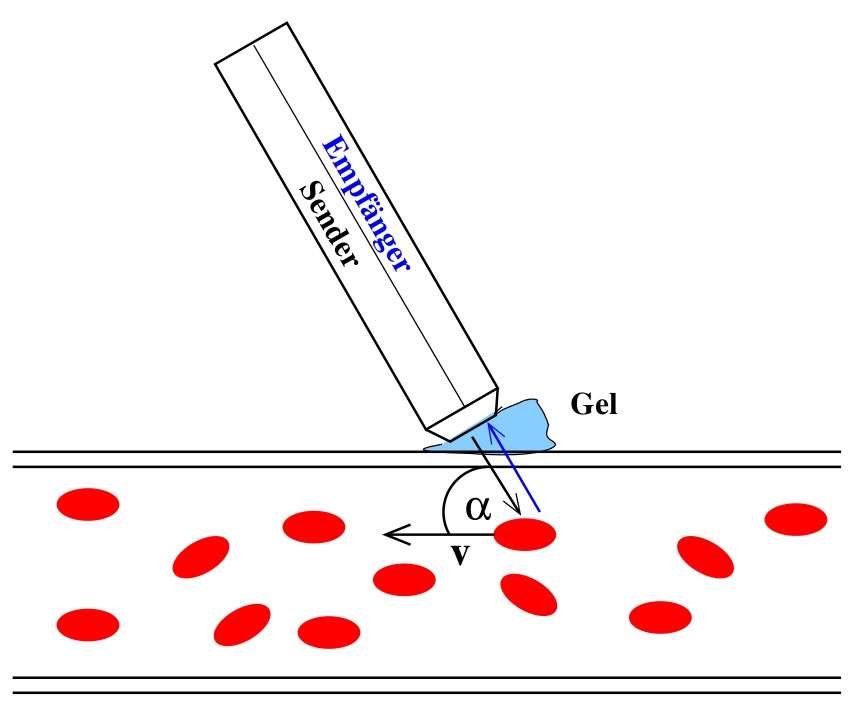
\includegraphics[width=0.75\linewidth]{content/data/ultraschall_schematisch.jpg}
    \caption{Eine schematische Darstellung einer Untersuchung von Blutströmungen mit einem Ultraschallgerät. \cite[1]{anleitung}}
    \label{fig:ultraschall_schematisch}
\end{wrapfigure}
Die Frequenzverschiebung wird durch
\begin{equation*}
    \Delta \nu = \nu_0 \frac{v}{c} \left ( \cos \alpha + \cos \beta \right )
\end{equation*}
beschrieben, wobei $\alpha$ und $\beta$ die Winkel zwischen der Geschwindigkeit $v$ und der Wellennormale sind.
In diesem Versuch (bzw. bei dem verwendeten Impuls-Echo-Verfahren) gilt $\alpha = \beta$ und es folgt für die Frequenzverschiebung
\begin{equation}
    \Delta \nu = 2 \nu_0 \frac{v}{c} \cdot \cos \alpha \, .
    \label{eqn:frequenzverschiebung}
\end{equation}
\\
Ultraschall kann auf verschiedenen Wegen erzeugt werden.
Eine Methode ist die Nutzung des piezo-elektrischen Effekts.
Befindet sich ein piezo-elektrischer Kristall in einem elektrischen Wechselfeld und eine polare Achse des Kristalls zeigt in Richtung des Feldes, dann wird dieser zum Schwingen angeregt.
Die Schwingung des Kristalls erzeugt Ultraschallwellen.\\
Stimmt die Anregungsfrequenz des elektrischen Feldes mit der Eigenfrequenz des Kristalls überein, kommt es zur Resonanz und es können große Schwingungsamplituden erzeugt werden.
Dabei entstehen hohe Schallenergiedichten die zur Untersuchung von Strömungen genutzt werden können.
\\
\\
Ein Piezokristall kann auch als Empfänger von Schallwellen genutzt werden.
Treffen Schallwellen auf den Kristall wird dieser zum Schwingen angeregt.
Durch die Schwingung wird der Kristall verformt und die elektrische Polarisation verändert.
Dies erzeugt eine elektrische Spannung, welche gemessen werden kann.\\
Am häufigsten werden Quarze als Piezokristall verwendet.
Die verwendete Ultraschallsonde in dem Versuch wird als Ultraschallsender und -empfänger genutzt.